\section{Анализ предметной области}
\subsection{История создания трёхмерной компьютерной графики}

Впервые трёхмерная компьютерная графика была реализована в 1960-х годах, когда Айван Сазерленд и Дэвид Эванс основали первую в мире кафедру компьютерной графики в университете Юты, США. Основой трёхмерной компьютерной графики стала Евклидова геометрия, а также все математические открытия, которые были сделаны до XX века. Первые трёхмерные изображения состояли из множества точек и кривых, определяемых математическим уравнением. Именно в то время появился прародитель для всех современных 3D-редакторов - программа Sketchpad.

Развитие трёхмерной графики шло быстрым ходом, и уже совсем скоро вместо векторной графики появилась возможность создавать и трёхмерные растровые изображения, а также использовать различные текстуры для объектов, обрабатывать их тени, и наконец - проводить компиляцию всего кода в готовое изображение.
\subsection{Основные принципы работы трёхмерной графики}

Главным основоположником систематизации математических аксиом и теорем в области геометрии был Евклид. Именно его труды способствовали разработке и технологическому прорыву трёхмерной графики в XX веке. Но за её развитием стоит не только сам Евклид, а также и другие великие умы и открытия, как например, формулы Виета для нахождения корней квадратичного уравнения, благодаря чему в символьном анализе алгебры неизвестные переменные обозначаются как x, y и z, а коэффициенты - a, b и c. А основой отсчёта  пространства стала система трёхмерных координат Декарта.

Также незаменимый влкад в разработку трёхмерной графики и геометрии внесли Российские учёные XX века - Борис Делоне и Георгий Вороной. Борис Делоне предложил метод «Триангуляции Делоне», которая стала основой формирования граней трёхмерных моделей, а Георгий Вороной создал «Диаграмму Вороного», которая используется до сих пор в картографических софтах, дизайне и трёхмерной графике.

Любая трёхмерная модель объекта математически находится в трёх измерениях. И если, чтобы отрисовать изображение объекта в двух измерениях компьютерной мощи требовалось не так много, то с добавлением третьего измерения - оси Z, требовательность к производительности компьютерного железа резко возрасла.

Трёхмерные объекты математически представляются в виде множества точек - вершин, и в тоже время они, соединенные отрезками, образуют рёбра фигиры, а множество рёбер на одной плоскости образуют поверхности - грани фигуры. Данный массив точек трансформируется с учётом матрицы перспективы камеры, далее - накладываются текстуры на поверхности граней фигуры - изображения также растягивают и трансформируют с учётом перспективы наклона грани, затем - обрабатывают свет, падающий на модель, путём изменения яркости текстуры граней, в зависимости от источников света, и наконец - добавляют тень, которая отбрасывает данная трёхмерная модель.

\subsection{Работа с OpenGL}

"OpenGL" (Open Graphics Library) - это кроссплатформенная спецификация, независимая от языка программирования, которая определяет программный интерфейс для написания приложений для двумерной и трёхмерной компьютерной графики. По своей сути, OpenGL - это низкоуровневый API, который позволяет напрямую работать с коммандами и буфферами видеокарты, так что для его использования необходимо иметь хотя бы основные понимания работы трёхмерной графики и линейной алгебры. Для простого начала знакомства и использования спецификации OpenGL существует множество официальных готовых эффективных реализаций для Windows, Unix-платформ и MacOS.

Спецификация OpenGL была создана в эпоху активного распространения компьютерных 3D игр и приложений, когда взникла сложность с совместимостью устройств во время реализации компьютерного кода при использовании различных аппаратных устройств - процессоров, видеоадаптеров, устройств хранения информации и материнской платы. Это вызывало сильные затраты, трудности и замедляло разработку программного обеспечения. Поэтому, компания Silicon Graphics - лидирующая в то время в сфере производства оборудования для обработки трёхмерной графики разработала программный интерфейс, целью которого было систематизировать доступ и обработку трёхмерных моделей на аппаратном уровне. Плодами их трудов стала спецификация OpenGL, который стандартизировал обработку различных функций 3D систем, которые выполняли единые команды из списка доступных, согласно установленной программой спецификации, что позволило создавать программное обеспечение, которое одинаково корректно работает на всех видах графического оборудования.

Принцип работы  OpenGL заключается в получении геометрических векторных примитивов и построении растровой картинки в памяти видеокарты и выводе её на экран. Из-за своей низкоуровневости, данная спецификация требует диктовать программе точный порядок действий от программиста и использовать императивный подход в разработке приложений. Но несмотря на эти сложности, это даёт большой простор, гибкость и свободу в создании программ.

Последняя вышедшая версия OpenGL 4.6, в данный момент уже считается устаревшей, и на смену ей пришёл современный и оптимизированный для новых видеокарт API Vulcan, который стал прямым преемником OpenGL.

\subsubsection{Функции и операторы OpenGL}
Все функции OpenGL можно разделить на пять категорий:
\begin{itemize}
	\item функции описания примитивов определяют объекты нижнего уровня иерархии (примитивы), которые способна отображать графическая подсистема. В OpenGL в качестве примитивов выступают точки, линии, многоугольники и т.д;
	\item функции описания источников света служат для описания положения и параметров источников света, расположенных в трехмерной сцене;
	\item функции задания атрибутов. С помощью задания атрибутов программист определяет, как будут выглядеть на экране отображаемые объекты. Другими словами, если с помощью примитивов определяется, что появится на экране, то атрибуты определяют способ вывода на экран. В качестве атрибутов OpenGL позволяет задавать цвет, характеристики материала, текстуры, параметры освещения;
	\item функции визуализации позволяют задать положение наблюдателя в виртуальном пространстве, параметры объектива камеры. Зная эти параметры, система сможет не только правильно построить изображение, но и отсечь объекты, оказавшиеся вне поля зрения;
	\item набор функций геометрических преобразований позволяют программисту выполнять различные преобразования объектов – поворот, перенос, масштабирование.
\end{itemize}

При этом OpenGL может выполнять дополнительные операции, такие как использование сплайнов для построения линий и поверхностей, удаление невидимых фрагментов изображений, работа с изображениями на уровне пикселей и т.д.

\subsubsection{Интерфейс OpenGL}
OpenGL состоит из набора библиотек. Все базовые функции хранятся в основной библиотеке, для обозначения которой в дальнейшем будеn использоваться аббревиатура GL. Помимо основной, OpenGL включает в себя несколько дополнительных библиотек.

Первая из них – библиотека утилит GL(GLU – GL Utility). Все функции этой библиотеки определены через базовые функции GL. В состав GLU вошла реализация более сложных функций, таких как набор популярных геометрических примитивов (куб, шар, цилиндр, диск), функции построения сплайнов, реализация дополнительных операций над матрицами и т.п.

OpenGL не включает в себя никаких специальных команд для работы с окнами или ввода информации от пользователя. Поэтому были созданы специальные переносимые библиотеки для обеспечения часто используемых функций взаимодействия с пользователем и для отображения информации с помощью оконной подсистемы. Наиболее популярной является библиотека GLUT (GL Utility Toolkit). Формально GLUT не входит в OpenGL, но включается почти во все его дистрибутивы и имеет реализации для различных платформ. GLUT предоставляет только минимально необходимый набор функций для создания OpenGL-приложения. Функционально аналогичная библиотека GLX менее популярна. В дальнейшем в этом пособии в качестве основной будет рассматриваться GLUT.

\begin{figure}[H]
	\center{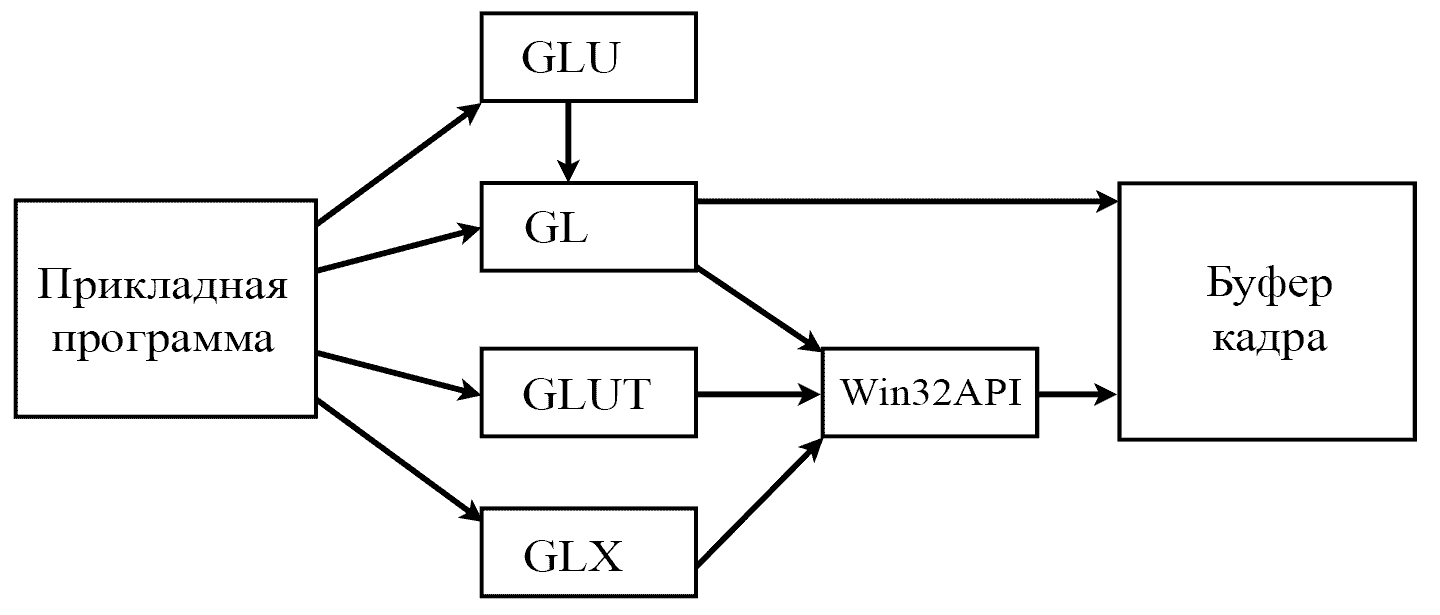
\includegraphics[width=1\linewidth]{diagram6.png}}
	\caption{Организация библиотеки OpenGL}
	\label{diagram6:image}
\end{figure}

Функции, специфичные для конкретной оконной подсистемы, обычно входят в ее прикладной программный интерфейс. Так, функции, поддерживающие выполнение OpenGL, есть в составе Win32 API и X Window. На рисунке схематически представлена организация системы библиотек в версии, работающей под управлением системы Windows. Аналогичная организация используется и в других версиях OpenGL.

\subsubsection{Архитектура OpenGL}

Функции OpenGL реализованы по принципу клиент-сервер. Приложение выступает в роли клиента – оно посылает команды, а сервер OpenGL интерпретирует и выполняет их. Сам сервер может находиться как на том же компьютере, на котором находится клиент (например, в виде динамически загружаемой библиотеки – DLL), так и на другом (при этом может быть использован специальный протокол передачи данных между машинами).

GL обрабатывает и рисует в буфере кадра графические примитивы с учетом некоторого числа выбранных режимов. Каждый примитив – это точка, отрезок, многоугольник и т.д. Каждый режим может быть изменен независимо от других. Определение примитивов, выбор режимов и другие операции описываются с помощью команд в форме вызовов функций прикладной библиотеки.

Примитивы определяются набором из одной или более вершин (vertex). Вершина определяет точку, конец отрезка или угол многоугольника. С каждой вершиной ассоциируются некоторые данные (координаты, цвет, нормаль, текстурные координаты и т.д.), называемые атрибутами. В подавляющем большинстве случаев каждая вершина обрабатывается независимо от других.

С точки зрения архитектуры графическая система OpenGL является конвейером, состоящим из нескольких последовательных этапов обработки графических данных.

Команды OpenGL всегда обрабатываются в том порядке, в котором они поступают, хотя могут происходить задержки перед тем, как проявится эффект от их выполнения. В большинстве случаев OpenGL предоставляет непосредственный интерфейс, т.е. определение объекта вызывает его визуализацию в буфере кадра.

С точки зрения разработчиков, OpenGL – это набор команд, которые управляют использованием графической аппаратуры. Если аппаратура состоит только из адресуемого буфера кадра, тогда OpenGL должен быть реализован полностью с использованием ресурсов центрального процессора. Обычно графическая аппаратура предоставляет различные уровни ускорения: от аппаратной реализации вывода линий и многоугольников до нестандартных и непривычных графических процессоров с поддержкой множеств операций над геометрическими данными.

\begin{figure}[H]
	\center{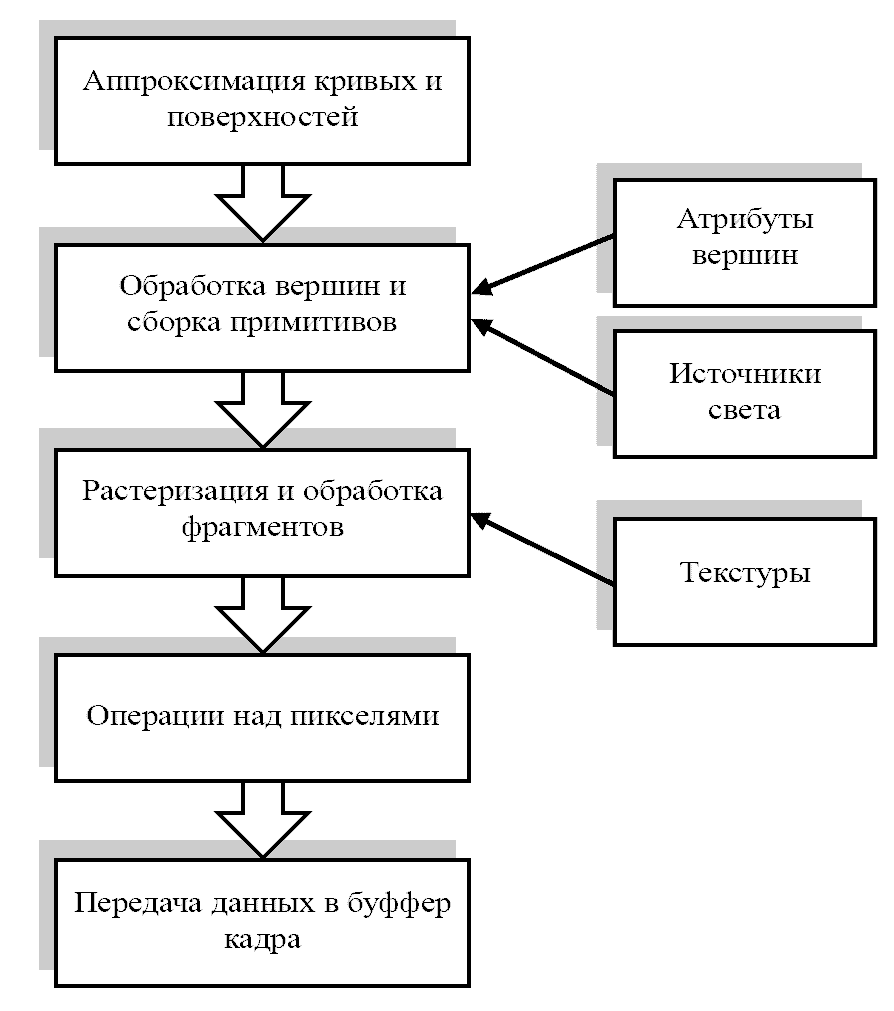
\includegraphics[width=0.7\linewidth]{diagram7.png}}
	\caption{Функционирование конвейера OpenGL}
	\label{diagram7:image}
\end{figure}

OpenGL является соединяющим звеном между аппаратурой и пользовательским уровнем, что позволяет предоставлять единый интерфейс на разных платформах, используя возможности аппаратной поддержки.

Кроме того, OpenGL можно рассматривать как конечный автомат, состояние которого определяется множеством значений специальных переменных и значениями текущей нормали, цвета, координат текстуры и других атрибутов и признаков. Вся эта информация будет использована при поступлении в графическую систему координат вершины для построения фигуры, в которую она входит. Смена состояний происходит с помощью команд, которые оформляются как вызовы функций.

\subsubsection{Работа с OpenTK}

OpenTK (Open набор средств) — это расширенная низкоуровневая библиотека C\#, которая упрощает работу с OpenGL, OpenCL и OpenAL. OpenTK можно использовать для игр, научных приложений или других проектов, требующих трехмерной графики, аудио или вычислительной функциональности.

Использование OpenTK предоставляет следующие возможности:
\begin{itemize}
	\item Быстрая разработка — OpenTK предоставляет надежные типы данных и встроенную документацию для улучшения рабочего процесса программирования и перехвата ошибок проще и быстрее;
	\item Простая интеграция — OpenTK была разработана для легкой интеграции с приложениями .NET;
	\item Разрешительная лицензия — OpenTK распространяется в соответствии с лицензиями MIT/X11 и полностью бесплатно;
	\item Расширенные привязки type-Сейф — OpenTK поддерживает последние версии OpenGL, OpenGL|ES, OpenAL и OpenCL с автоматической загрузкой расширений, проверка проверка и встроенной документацией;
	\item Гибкие параметры графического интерфейса — OpenTK предоставляет собственное, высокопроизводительные окно игры и приложения;
	\item Полностью управляемый, CLS-совместимый код . OpenTK поддерживает 32-разрядные и 64-разрядные версии macOS без неуправляемых библиотек;
	\item Трехмерные математические набор средств поставки Quaternion Vector Matrix OpenTK и Bezier структуры с помощью 3D-математических набор средств.
\end{itemize}

\subsection{Математика освещения в трёхмерной графике}

Для того, чтобы воссоздать искусственное освещение внутри моделируемого виртуального пространства, нам необходимо смоделировать поведение света при взаимодействии с различными поверхностями. Интересно, что эту задачу начал решать ещё в далеком в 18-м веке человек по имени Иоганн Генрих Ламберт.

В 1760 году швейцарский учёный выпустил книгу под названием Photometria. В ней он изложил фундаментальные правила поведения света; самым примечательным из них стало следующее — поверхность испускает свет (отражением или как источник освещения) таким образом, что яркость испускаемого света меняется в зависимости от косинуса угла между поверхностью нормали и наблюдателем.

\begin{figure}[H]
	\center{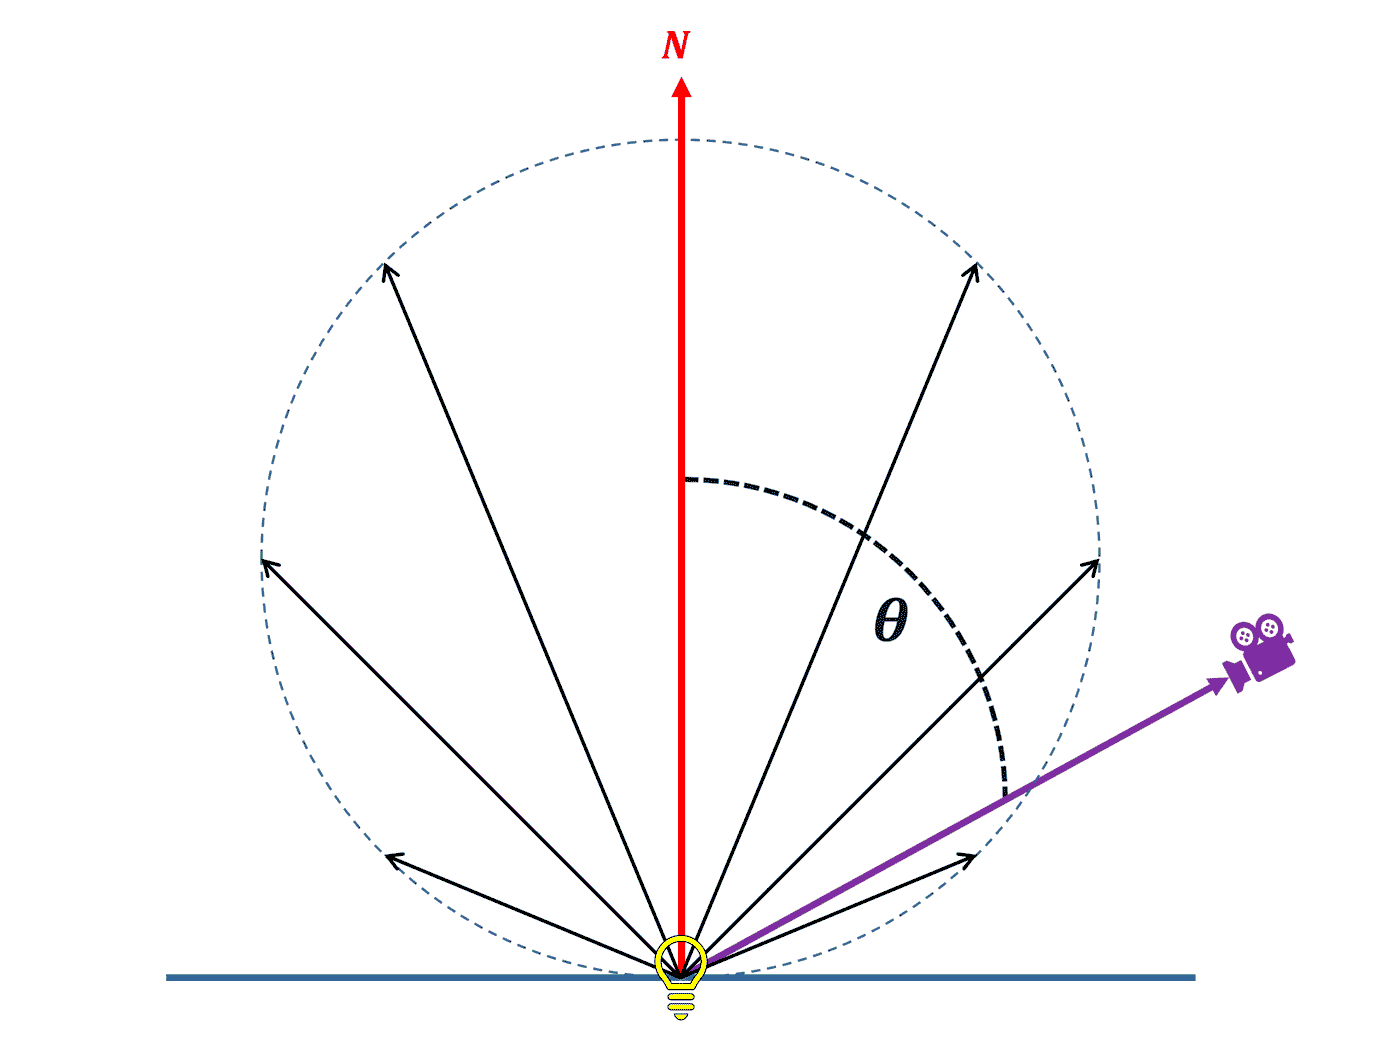
\includegraphics[width=0.8\linewidth]{diagram9.png}}
	\caption{Зависимость яркости отражаемого света поверхности от косинуса угла между нормалью и наблюдателем}
	\label{diagram9:image}
\end{figure}

\subsubsection{Рассеянный свет}

Это простое правило заложило основание определению рассеянного (diffuse light) освещения. Это математическая модель, используемая для вычисления цвета поверхности в зависимости от её физических свойств (например, её цвета и степени отражения света) и расположения источника освещения.

При 3D-визуализации для этого требуется некоторое множество параметров, что можно представить в виде такой схемы на рисунке ~\ref{diagram10:image}.

\begin{figure}[H]
	\center{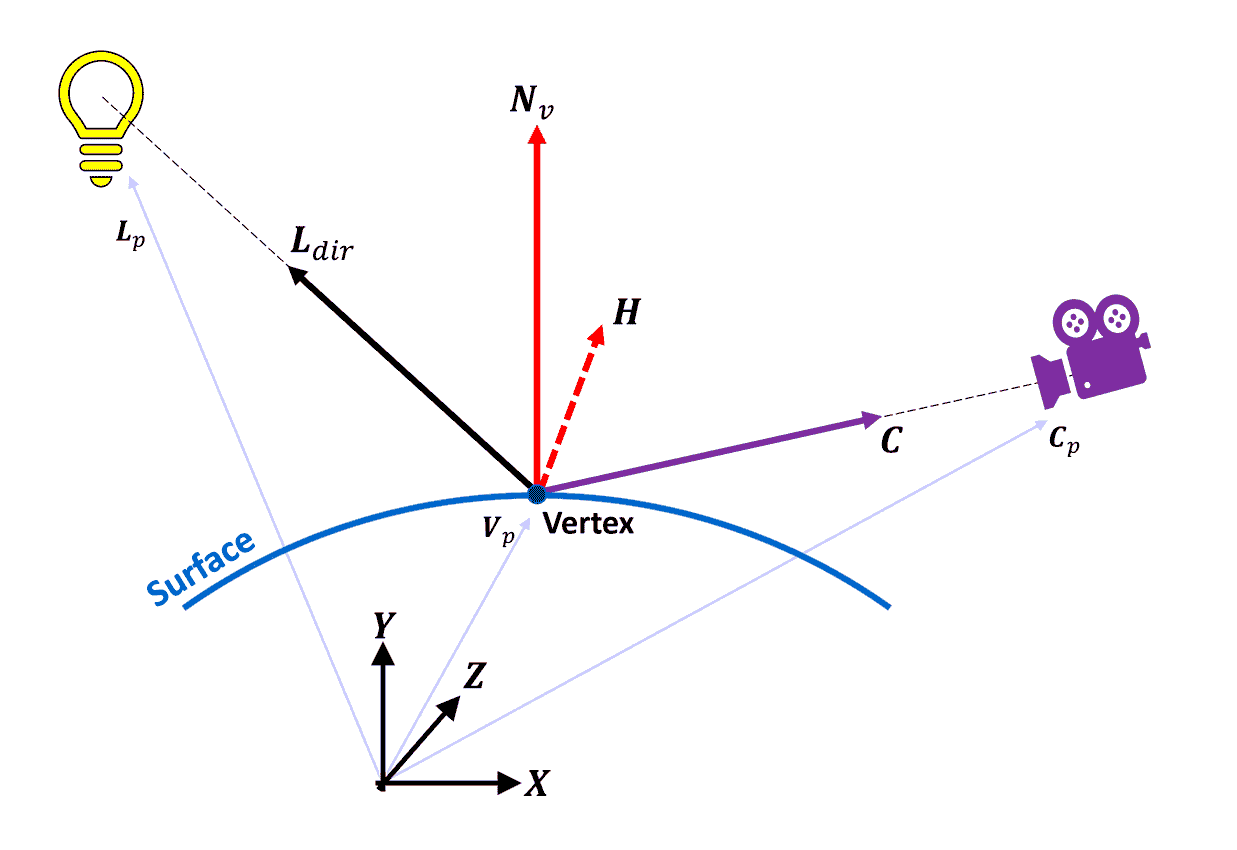
\includegraphics[width=0.8\linewidth]{diagram10.png}}
	\caption{Схема используемых параметров при 3D-рендеринге освещения}
	\label{diagram10:image}
\end{figure}

На изображении показано много указателей, это векторы, и для вычисления цвета отражения требуются следующие векторы:
\begin{itemize}
	\item 3 вектора для позиции вершины, источника освещения и камеры, смотрящей на сцену;
	\item 2 вектора для направлений источника освещения и камеры с точки зрения вершины;
	\item 1 вектор нормали (изображён красным);
	\item 1 полувектор (он всегда посередине между векторами направлений освещения и камеры).
\end{itemize}

Они вычисляются на этапе обработки вершин процесса рендеринга, а объединяющее их всех уравнение  (называемое ламбертовой моделью) (формула ~\ref{form1:equation}):

\begin{equation}
	\fontsize{17}{20}{L_{D} = \sum_{0}^{n}(C_{S} × C_{L} × (\hat{N}_{\nu} · \hat{L}_{dir}) × A × S)}
	\label{form1:equation}
\end{equation}

То есть, цвет вершины при рассеянном освещении вычисляется перемножением цвета поверхности, цвета источника освещения и скалярного произведения векторов нормали вершины и направления света с коэффициентами затухания и прожекторного освещения. Эта операция выполняется для каждого источника освещения в сцене, отсюда и символ суммы в начале уравнения.

Всё это нужно для вычисления значения рассеянного освещения и все эти операции требуется выполнять для каждого источника освещения в виртуальной сцене, или, по крайней мере, для каждого источника, который существует на сцене и обрабатывается программой. Многие из этих уравнений выполняются графическими API, но их можно выполнять и вручную, если необходимо реализовывать более сложные операции над изображением.

\subsubsection{Общий свет}

Но помимо рассеянного света существует бесконечное множество других видов освещений, и каждая поверхность отражает свет, поэтому все они влияют на общее освещение сцены. Даже ночью присутствует фоновое освещение, будь то звёзды и планеты или свет, рассеивающийся в атмосфере.

Для моделирования реалистичного света, вычисляется ещё одно значение освещения: ambient lighting  (освещение окружающей среды) (формула ~\ref{form2:equation}), или же общий свет.

\begin{equation}
	\fontsize{17}{20}{L_{A} = C_{SA} × \left(C_{GA} + \sum_{0}^{n}(A × S × C_{LA})\right)}
	\label{form2:equation}
\end{equation}

Это уравнение проще, чем для рассеянного освещения, потому что не требуются направления. Здесь выполняется простое перемножение различных коэффициентов:

\begin{itemize}
	\item C$_S$$_A$ — цвет подсветки поверхности
	\item C$_G$$_A$ — цвет подсветки глобальной 3D-сцены
	\item C$_L$$_A$ — цвет подсветки всех источников освещения в сцене
\end{itemize}

\subsubsection{Отраженный свет}

Определив фоновое освещение и введя в расчет рассеянный свет источников освещения от различных поверхностей 3D-мира, виртуальное освещение начинает выглядеть намного более реалистично. Но модель Ламберта работает только для материалов, которые отражают освещение от своей поверхности во всех направлениях. Объекты, изготовленные из стекла или металла, создают другой тип отражения, называемый зеркальным (specular). И для него тоже необходимо определить уравнение (~\ref{form3:equation}).

\begin{equation}
	\fontsize{17}{20}{L_{S} = C_{S} × \sum_{0}^{n} \left(C_{LS} × (\hat{N}_{\nu} · \hat{H})^{p} × A × S\right)}
	\label{form3:equation}
\end{equation}

Отдельные части этой формулы уже были определены раннее: имеется два значения зеркального цвета (одно для поверхности — C$_{S}$, другое для света — C$_{LS}$), а также привычные коэффициенты затухания и прожекторности.

Так как зеркальное отражение очень сфокусировано и направлено, для определения яркости зеркального освещения используются два вектора: нормаль вершины и полувектор. Коэффициент $p$ называется мощностью зеркального отражения, это число, определяющее яркость отражения в зависимости от свойств материала поверхности. При увеличении $p$ зеркальный эффект становится ярче, но более сфокусированным и меньшим по размерам.

\subsubsection{Испускаемый свет}

Последний учитываемый элемент — самый простой, потому что математически представляется лишь одним числом. Оно называется испускаемым (emissive) освещением, и применяется к объектам, являющимся непосредственным источником освещения, то есть к пламени, фонарику или Солнцу.

Это означает, что на данный момент определены одно число и три набора уравнений для вычисления цвета вершины поверхности, учёта фонового освещения (окружающей среды), а также взаимодействия между различными источниками освещения и свойствами материала поверхности (diffuse и specular). В программной среде можно использовать либо только один или же скомбинировать все четыре источника света, просто сложив их вместе (формула ~\ref{form4:equation}):

\begin{equation}
	\fontsize{17}{20}{L_{O} = L_{D} + L_{A} + L_{S} + L_{E}}
	\label{form4:equation}
\end{equation}

Визуально сочетание различных видов света выглядит так:

\begin{figure}[H]
	\center{\hspace{10mm}{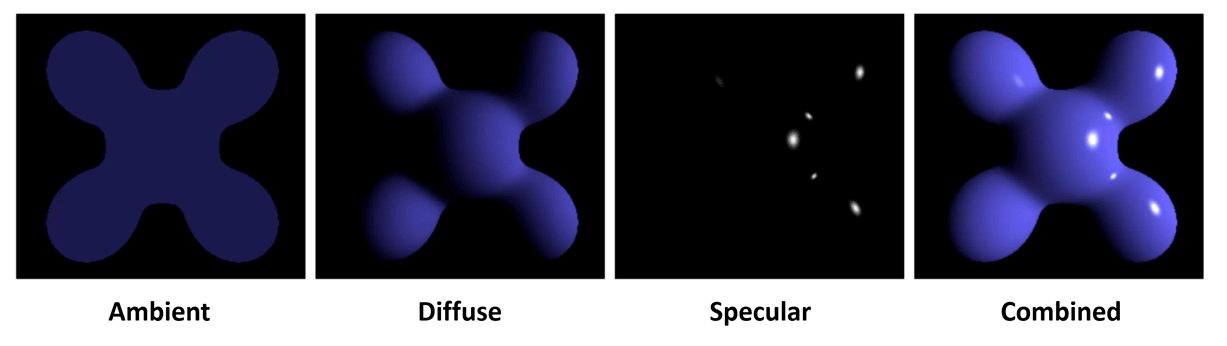
\includegraphics[width=1\linewidth]{diagram11.png}}}
	\caption{Визуальное представление результата наложения нескольких типов освещений на одном объекте}
	\label{diagram11:image}
\end{figure}

\subsection{Аффинные преобразования трёхмерного пространства}

При работе с трёхмерными объектами, часто требуется совершать по отношению к ним различные преобразования: двигать, поворачивать, сжимать, растягивать, скашивать и т.д. При этом в большинстве случаев требуется, чтобы после применения этих преобразований сохранялись определенные свойства.

Преобразование плоскости называется аффинным (от англ. affinity – родство), если
\begin{itemize}
	\item оно взаимно однозначно;
	\item образом любой прямой является прямая.
\end{itemize}

Преобразование называется взаимно однозначным, если
\begin{itemize}
	\item разные точки переходят в разные;
	\item в каждую точку переходит какая-то точка.
\end{itemize}

Свойства аффинного преобразования в трехмерном пространстве:
\begin{itemize}
	\item отображает n-мерный объект в n-мерный: точку в точку, линию в линию, поверхность в поверхность;
	\item сохраняет параллельность линий и плоскостей;
	\item сохраняет пропорции параллельных объектов – длин отрезков на параллельных прямых и площадей на параллельных плоскостях.
\end{itemize}

Любое аффинное преобразование задается матрицей 3x3 с ненулевым определителем (формула ~\ref{form6:equation}) и вектором переноса (формула ~\ref{form5:equation}):

\begin{equation}
	\fontsize{17}{20}{
	\vec{p_{'}} = R\vec{p} + \vec{t}}
	\label{form5:equation}
\end{equation}

\begin{equation}
	\fontsize{17}{20}{
	\left(
	\begin{matrix}
		x^{'} \\
		y^{'} \\
		z^{'}
	\end{matrix}
	\right)
	=
	\left(
	\begin{matrix}
		R_{11} & R_{12} & R_{13}\\
		R_{21} & R_{22} & R_{23}\\
		R_{31} & R_{32} & R_{33}
	\end{matrix}
	\right)
	\left(
	\begin{matrix}
		x\\
		y\\
		z
	\end{matrix}
	\right)
	+
	\left(
	\begin{matrix}
		t_{x}\\
		t_{y}\\
		t_{z}
	\end{matrix}
	\right)}
	\label{form6:equation}
\end{equation}

\subsubsection{Параллельный перенос}
\begin{figure}[H]
	\center{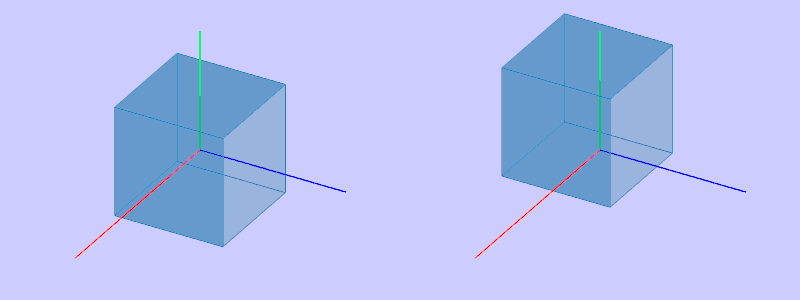
\includegraphics[width=1\linewidth]{prim1.png}}
	\caption{Преобразование вида параллельный перенос}
	\label{prim1:image}
\end{figure}

Матрица этого преобразования выглядит следующим образом:

\begin{equation}
	\fontsize{17}{20}{\left(
	\begin{matrix}
		1 & 0 & 0 & t_{x}\\
		0 & 1 & 0 & t_{y}\\
		0 & 0 & 1 & t_{z} \\
		0 & 0 & 0 & 1
	\end{matrix}
	\right)}
\end{equation}

В данном случае матрица R = E, единичной матрице.

\subsubsection{Поворот вокруг оси}
\begin{figure}[H]
	\center{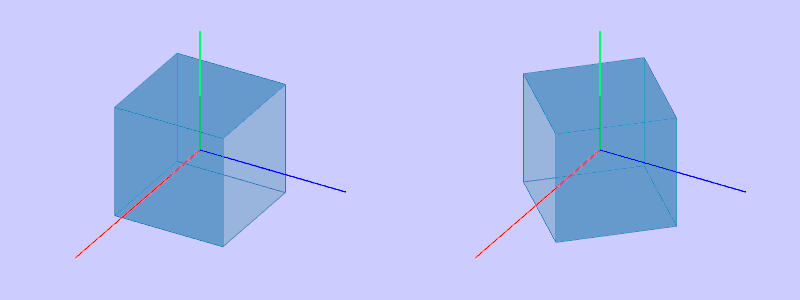
\includegraphics[width=1\linewidth]{prim2.png}}
	\caption{Преобразование вида поворот вокруг оси}
	\label{prim2:image}
\end{figure}

Заметим, что при повороте вокруг оси y ординаты точек (у-координаты) не меняются. Также стоит отметить, что координаты x и z точки преобразуются независимо от y-координаты. Это означает, что любая точка p(x, y, z) перейдет в точку p’(x’(x, z), y, z’(x, y)). Теперь осталось понять, как преобразуются координаты x и z: в плоскости Oxz это будет поворот вокруг начала координат по часовой стрелке (т.к. x z y - левая тройка), т.е. в отрицательном направлении. Матрица такого преобразования известна:

\begin{equation}
	\fontsize{17}{20}{
	\left(
	\begin{matrix}
		\cos (-\phi_{y}) & -\sin(-\phi_{y}) \\
		\sin (-\phi_{y}) & \cos (-\phi_{y})
	\end{matrix}
	\right)}
\end{equation}

\vspace*{5mm}Матрица преобразования Ry(φy):

\begin{equation}
	\fontsize{17}{20}{
		\left(
		\begin{matrix}
			\cos (-\phi_{y}) & -\sin(-\phi_{y}) \\
			0 & 1 & 0 \\
			\sin (-\phi_{y}) & \cos (-\phi_{y})
		\end{matrix}
		\right)}
\end{equation}

\subsubsection{Масштабирование}
\begin{figure}[H]
	\center{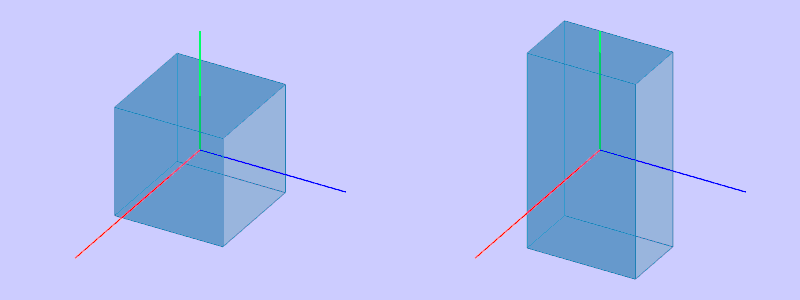
\includegraphics[width=1\linewidth]{prim3.png}}
	\caption{Преобразование вида масштабирование}
	\label{prim3:image}
\end{figure}

Коэффициенты сжатия/растяжения, по аналогии с двухмерным пространством, определяются диагональными членами матрицы R (формула ~\ref{form10:equation}).

\begin{equation}
	\fontsize{17}{20}{
		\left(
		\begin{matrix}
			S_{x} & 0 & 0 \\
			0 & s_{y} & 0 \\
			0 & 0 & s_{z}
		\end{matrix}
		\right)}
	\label{form10:equation}
\end{equation}

\vspace*{5mm}Результат:

\begin{equation}
	\fontsize{17}{20}{
		\begin{matrix}
			x^{'} = s_{x}x \\
			y^{'} = s_{y}y \\
			z^{'} = s_{z}z
		\end{matrix}}
	\label{form11:equation}
\end{equation}

Комбинация коэффициентов $s_x$ = -1, $s_y$ = 1, $s_z$ = 1 будет задавать отражение от плоскости Oyz (x = 0). При $s_x$ = $s_y$ = $s_z$ = -1 получим центральную симметрию относительно начала координат.